\chapter{Encaminhamento da solução}

Com o intuito de testar os efeitos de envelhecimento em sistemas embarcados nós tecnológicos diferentes foi escolhido o desenvolvimento de osciladores em anel utilizando alguma linguagem de descrição de hardware (VHDL ou Verilog).

Os dois FPGAs testados serão o Cyclone IV (CMOS de 60nm) e o Kintex-7 (CMOS de 28nm), escolhidos por sua disponibilidade no Laboratório de Processamento de Sinais e Imagem. Também é desejado realizar os testes com um FPGA de tecnologia FinFET, porém não há disponibilidade deles no laboratório, então seu ensaio depende de empréstimo de outro departamento.

Os ensaios de envelhecimento serão realizados em uma câmara térmica disponível no Laboratório de Caracterização Elétrica.

Etapas do trabalho:
\begin{itemize}
    \item Desenvolvimento e testes do Oscilador em Anel para o Cyclone IV
    \item Desenvolvimento e testes do Oscilador em Anel para o Kintex-7
    \item Validação dos circuitos desenvolvidos
    \item Medidas antes do envelhecimento
    \item Ensaios de envelhecimento acelerado
    \item Medidas depois do envelhecimento e análise de dados
\end{itemize}

Fluxograma:
\begin{figure}[H]
    \centering
    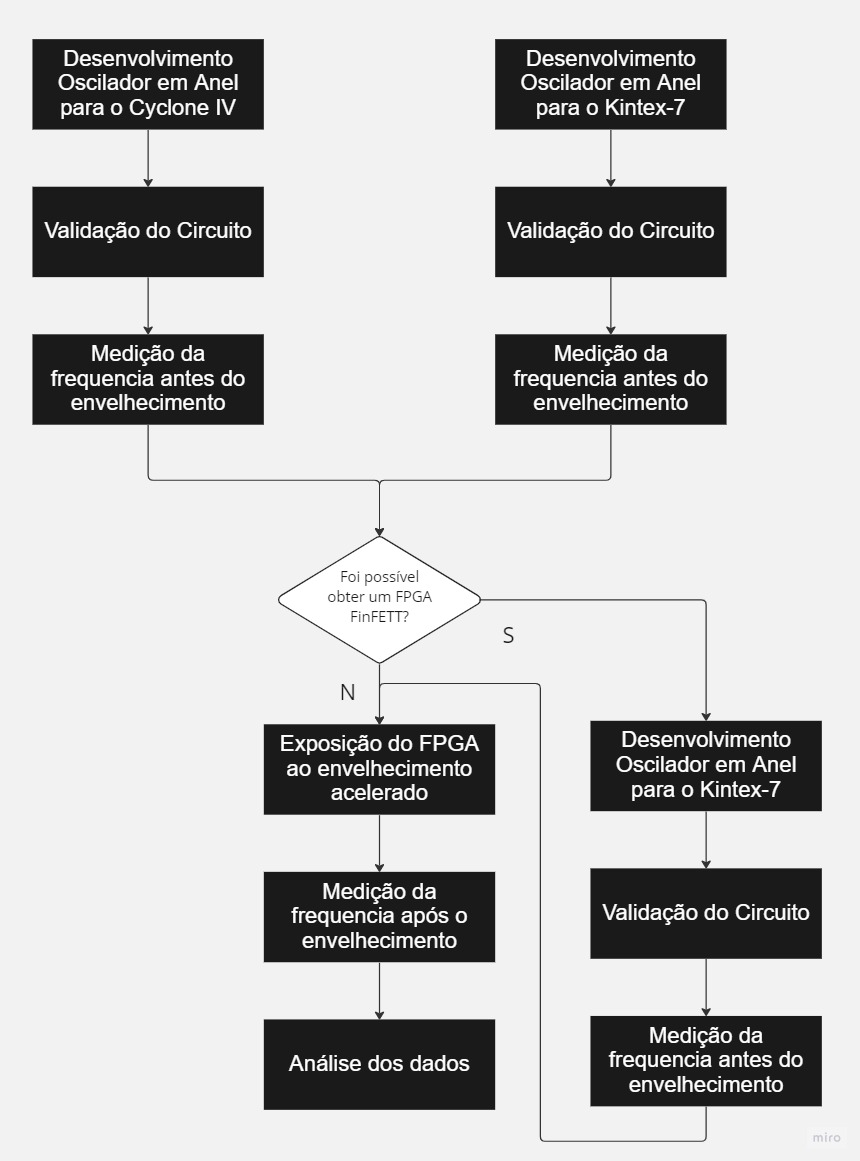
\includegraphics[width=\linewidth]{figures/Flowchart.jpg}
    \caption{Fluxograma. Fonte: O autor}
    \label{fig:Flowchart}
\end{figure}